% !TEX encoding = UTF-8 Unicode
%!TEX root = thesis.tex
% !TEX spellcheck = en-US
%%=========================================
\chapter[Bot Metrics]{Do bots,  make click, text and behavior metrics irrelevant?}

\section{What are bots and how are they used?}
In general, bots are types of software which run automated tasks(which are repetitive and allows for the program to be faster at doing some tasks than what normal humans would be able to. There are many types of bots, for example gaming bots which can be programmed to efficiently react faster than what a human would be able to on certain events in the game, thus making the humans better players. Others examples include auction bots, which hunt for bargains. Ebay went to court in 2000( \cite{Computerworld:Ebay}) in order to stop this type of behavior, the federal courts in turn then decided to block Bidders Edge and their bots from accessing Ebays API.
\\

In the US 2010 mid-term election, social bots were reportedly used to influence the support of some candidates while effectively slandering others by tweeting thounsands of tweets which pointed to websites which contained fake news about the other candidate (\cite{ICWSM112850}). This example highlights the potential seriousness of social bots. 
\\
It is not only in elections these bots have a great influence, during the aftermath of the Boston bombings it was noted that social media(and bots) had a great effect on getting the message out there(\cite{Cassa:Twitter}), but there was also a negative effect which bots attributed on Twitter by re-tweeting peoples' unverified accusations or even checking out the credibility of the source, causing more hurt than good. \\
\\
Furthermore bots are used to mimic human activity, in for example service applications which appear to be human interaction but is instead a bot which for example tries to "help" you based on keywords. Bots are used in many areas, but are probably most known for their maliciousness in areas such as spam, bandwidth-thiefs, scrapers, worms and viruses as well as as nodes in a larger scale bot-nets is used for example for DDOS. These bots can be part of bigger bot-nets in order to for example generate revenue through for example click fraud. 
\\
\\
The observers article on fake traffic \cite{Observer:FakeTRAF} describes the problem and its extent: 
\begin{quote}
A recent study by comScore found that 54 percent of display ads shown in thousands of campaigns between May 2012 and February 2013 never appeared in front of a human being. Rather, the traffic came from bots. As an advertiser, this would be like buying a billboard you were told was seen by thousands of cars a day only to find out that was because the billboard sat next to the assembly line at a Ford plant. Sure, that’s a lot of cars, but there’s no one in them.
\\
\\
In fact, the system is so broken that, for some publishers, knowingly buying traffic that comes from bots is part of their business model. An anonymous publishing executive, who claimed to be buying up to \$35,000 worth of traffic per day, recently told Digiday that for publishers running an arbitrage model, all that matters is profit; quality of traffic does not factor into the equation.
\newline \mbox{} \hfill \citet{Observer:FakeTRAF}
\end{quote}

This quote from comScore highlights a important point in today's society. How does click metrics influence us, and how are they used? Are they useless, can they be used to measure something even though results most likely have been contaminated? and how does this type of behavior influence the buyers decision? These and some others are the question I will answer during this chapter. 

I will also look into bots in social media, how they interact and how they spread in order to seem like normal users as well as interact as normal users. 
\section{What is  social media statistics, and how is it utilized?}
With the rise of social media use, social media marketing got a bigger foothold, allowing marketeers to interact with their buyers to a bigger degree, and it allowed the buyers to interact with their brands. Following this trend, many companies have big social media presences. Social media statistics allows the companies to closely monitor and narrow down their demographic and easily make specific content for a specific demographic. Furthermore, it allows for the company to get free publicity through what is called "organic reach" (getting exposure through users' activity in order to generate more clicks from users' contact) as well as for example paid reach(ads sent to a predefined demographic)
Social media statistics allows for all of this to happen, as \cite{Singh2013} mentions:
\begin{quotation}
Social Media statistics about audience likes and dislikes makes it plausible to employ "push marketing"-techniques to target audiences with advertisements that are relevant to their interests. Also, parameters such as click through rates or CTR can further quantify the success (or failure) of an advertising campaign. 
\end{quotation}
This type of push marketing, utilizes the information the users' themselves have provided to the mother service(e.g. Facebook), like for example metadata which gives a certain characteristic which allows them to be targeted by the broad filters which services like e.g. Facebook uses. 
\\
Businesses also utilizes what is called pull marketing, which is a little more subtle, e.g. referrals, social competitions("like and share" and get the \textit{chance} to win X") these methods can generate traction in social media, and be spread by word of mouth. 
\\
\\
But most notably, these types of metrics can be abused by bots.
\subsubsection*{An example of why metrics may be come obfuscated}
What happens to social media analytics in a business environment when bots enter the fray? Depending on the function of the bot, its behavior can vary greatly. If the bot is what is called a crawler, the bot will crawl through real peoples feed and try to mimic their behavior, and then crawl and gather more data from other people in the first peoples feed and so on. This type of activity has atleast three types of repercussions, it firstly generates fake interest for other companies' social media analytics, it hides their original intention(liking "this page") and it likes "this page" and generates fake revenue and publicity.
\\
\\
A good real-life example is \cite{Symantec:Narang}, which had a set of inter chained accounts posing as real accounts in order to spread their own links about some dubious diet pills. The accounts stole meta data from real accounts. Instead of using compromised
accounts to tweet spam links, they were using accounts that impersonated brands and
celebrities. Symantec goes on to describe how they defined three types of accounts involved in this scam:
\begin{itemize}
\item {\textbf{Mockingbird}: Used real data from real celebrities for impersonating these individuals}
\item{\textbf{Parrot}: Fake accounts using stolen tweets and photographs of real women}
\item{\textbf{Egg}: New users with no set avatar}
\end{itemize}
Mockingbirds have the goal of promoting the weight loss tricks. These mockingbird-tweets would get thousands of likes from Parrot-accounts which spiders through the real accounts of the mockingbirds. Parrots then follow any and everyone in the hope that users will follow them back because they are using avatars of attractive women, a tactic that has proven very efficient. The Parrots have real content that they post each day which is fake, an not only the content of the Mockingbird, in order to seem more real. These tweets are usually stolen from real accounts in order to seem real.  The parrots will also engage in discussions and post "reviews" of the diet pills in order to make the diet pills seem more real while the egg accounts just inflate the like counts in order to make the mockingbirds as well as the parrots seem trustworthy. The egg accounts do not post any content, they just follow parrots.
\\
\\ The link provided by the mockingbirds seem real(with pictures of famous people). When a customer orders a free trial, they register the credit card and subsequently lose their money. 
\\
The point of this example is to show how easily for example likes can be misguiding for a company that tries to establish themselves as a brand within social media. 

\section{Do these metrics influence buyers?}
As we have seen, metrics can be obfuscated by many different factors; "click farms", bots, and other variables which can affect social media analytics. These factors may present in many different ways. In an article entitled "Beyond likes and tweets: Consumer engagement behavior and movie box office in social media", \cite{Oh2016}, they researched how consumer engagement behavior(CEB) was associated with economic performance based on popular movies released in the US. The study found that CEB in Facebook and YouTube correlated with gross-revenue in opening-week movies. The study further concluded that CEB played a pertinent role in relation to future economic performance, so in some cases pure metrics can have great effects on the consumer itself.
%%
%%
\\\\ Another good example of this is metrics in movies. In particular ratings on movies and Tv-series through IMDB(Internet movie data base), which is used to share users' opinions on films and tv-series in the form of ratings(top 250 movies, bottom 100) as well as recommendations and critics, both professional and user generated. In a paper entitled "Judgement devices and the evaluation of singularities: The use of performance ratings and narrative information to guide film viewer choice"(\cite{Bialecki2016}), the researchers noted that the use of metrics such as ratings(moviegoers set a threshold in which served as a "hurdle" in which movies they wanted to see had to pass). Research also indicated that if a movie had a high rating or were in the top 250 rating-list, it was likely moviegoers would see it because of the ratings themselves. Some subjects noted that the movie did not meet their expectations, but that they had to watch it because of the the ratings:
\begin{quotation}
\textbf{\textit{"}}I rented this movie on the strength of the ratings and glowing
reviews at this site [IMDb]. “Brilliant”,they said. “Dark and beautiful”,
they wrote. 8.4 stars. Well, all I can say is, these people
must have been on some serious drugs when [they] saw this
totally inane movie. . .I give this movie 1 black hole.\textbf{\textit{"}}
\newline \mbox{} \hfill \citet{Bialecki2016}
\end{quotation}


As we can conclude from \cite{Bialecki2016}, we can say that people buy largely based on word of mouth as well as from reviews or "click metrics" (in the form of stars on IMDB). While doing research for this article, I found several websites which both offered botting specifically for IMDB(increase in stars), as well as a direct example of a movie in which had been a "bottom 200-list"-er for a long time, and was considered one of the biggest movieflops, gathering great nominations such as "Worst picture", "worst screen ensamble" \cite{wiki:Oogieloves} as well as a IMDB rating of 2.0 according to a petition\cite{change:Oogieloves}. The petition goes on to describe how the rating of the movie suddenly skyrocketed in June of 2013. in \ref{IMDB:rate} we can see the weighting of votes, most of which are at 10, which is the highest. This seems peculiar given the accolades which the movie was given and the initial score as well as the sudden boom. The ramifications of such actions will be discussed in the discussion part of this paper. 

\begin{figure}[h]
\centering
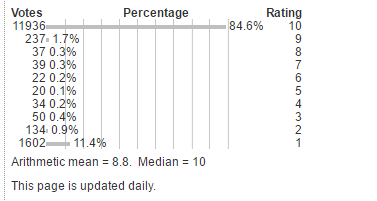
\includegraphics[scale=1]{imdbstats.PNG}
\caption{IMDB rating of movie in 2016, showing the skewed ratings.Courtesy of IMDB(\cite{IMDB:Oogieloves})}
\label{IMDB:rate}
\end{figure}

Another example of research done in this field is an article entitled "The Influence of Social Media: Twitter Usage Pattern during the 2014 Super Bowl Game" which analyzed how people used twitter during the superbowl event specifically looking at consumer interaction with advertisement.
The researchers used data mining in order to find correlations in data which may not be otherwise easily delectable. 
In the article(\cite{HyeonjeongShin2015}), the researchers asked two research questions: "How does the overall number of tweets differ between a game day and non-game day?"\cite{HyeonjeongShin2015}) and "What major topics in commercial related tweets were exchanged during the 2014 superbowl game?"\cite{HyeonjeongShin2015}). The data analysed for research question 1 (How does the overall number of tweets differ between a game day and non-game day?) indicated that Super bowl commercials created a buzz. The research also indicated that tweets about a commercial product accounted for 33\% of total commercial tweets generated on superbowl day(february 2) as opposed to 0.64\% and 9.48\% on january 26 and february 9th. Further, more than half of tweets(37 of 49 tweets) registered mentioned Budweiser products or their commercial. 
\\
\\
Even though these examples do not directly prove that consumers act on these type of data, one can draw the conclusion that user interacting might create a buzz and get your brand out there, thus leading to potentially more customers, subconsciously or otherwise. 

In the case of IMDB-ratings, they seem to influence what movies people want to see, and therefore revenue of movies which are featured in a popular way. This is backed up in a article entitled "An empirical investigation of user and system recommendations in e-commerce" about general statistics with e-commerce metrics \cite{Lin2014111} which could report that:
\begin{quote}
\begin{itemize}
\item {1\% increase in user recommendation volume increases product sales by 0.013\%.}
\item {1\% increase in user recommendation valence increases product sales by 0.022\%.}
\item {1\% increase in system recommendation strength increases product sales by 0.006\%.}
\end{itemize}
\end{quote}

\section{How can the statistics become irrelevant?}
With nearly 1.13 billion daily active users on Facebook \cite{FB:stats}, the importance of social media and how it influences people is important. As our lives gradually intertwine with social media and a personal digital presence, we become predisposed to marketing from friends and corporations.  But are we humans able to see the difference between what is user generated, or what is generated by bots or similar types of AI?
\\
\\
An article released in 2013, named "Is that a bot running the social media feed? Testing the differences in perceptions of communication quality for a human agent and a bot agent on Twitter"\cite{Edwards2014372} investigated the claim that humans would not see the difference between a bot, and a human in a single newsfeed on Twitter. They used a sample of 240 undergrad students enrolled in a communication course at a large mid-western research university with subjects ranging from the age of 18 to 39 years old. The researchers then used two treatment groups(the twitterbot and the human twitter agent). Those who chose to participate were given a link to a secure webpage with the study. After consenting to the study, the participants were randomly given one of the two twitter pages. The twitter profiles were designed to appear as information provided by the central for disease control(CDC) about sexually transmitted infections. The pages were identical all except for one important detail - the author; in the twitterbot case it was clearly stated that it was a CDC twitterbot, in the other case it was stated that the author was a CDC scientist. The study concluded that
 \begin{quote}
The findings demonstrate that Twitterbots can be viewed as credible, attractive,
competent in communication, and interactional, and might be an
appropriate program to transmit information in the social media
environment. 
\newline \mbox{} \hfill \citet{Edwards2014372}

\end{quote}
An article entitled "Globalization in social media and consumer relationships with brands in digital space" \cite{6959277120111201}, could conclude that 60\% of consumers\cite{6959277120111201} were strong brand advocates, and that they were more likely to buy the brand that they were advocates of. The paper continues to conclude that on a global basis, 18\% of users actively set up their online brand community\cite{6959277120111201}. 
\\
\\












